\documentclass[pdftex,12pt, letterpaper]{report}
\usepackage[spanish,activeacute]{babel}
\usepackage[utf8]{inputenc}
\usepackage{kpfonts} 

\usepackage{color}
\usepackage[pdftex]{graphicx}
\usepackage[letterpaper, total={8in,10in}]{geometry}
\newcommand{\HRule}{\rule{\linewidth}{0.5mm}}
    \usepackage[none]{hyphenat} 
% \graphicspath{{/home/carlosp/docencia/images/}}
\graphicspath{{images/}}

\begin{document}

\begin{titlepage}

\begin{center}


% \includegraphics[width=0.15\textwidth]{./logo}\\[1cm]    

% \textsc{\Large
% Quieres trabajar para tu tesis en  temas de vanguardia, usando herramientas
% de punta?\\[1cm]
% Trabaja en mecánica cuántica básica para resolver problemas 
% actuales. 
% }\\[1.5cm]

% \textsc{\Large Final year project}\\[0.5cm]
% \definecolor{backgroundcolor}{RGB}{}
% \definecolor{backgroundcolor}{RGB}{}
\definecolor{backgroundcolor}{RGB}{143,188,143}
\definecolor{backgroundcolor}{RGB}{255,228,196}
% \definecolor{backgroundcolor}{RGB}{255,0,0}
\pagecolor{backgroundcolor}
% Title
\HRule \\[0.0cm]
{ \Large \bfseries 
Temas Selectos de Física Computacional II
% Temas Selectos de Física Matemática y Teórica III
% Temas Selectos de Física Computacional III
\\[.5cm]
% \LARGE 
\Huge
Información cuántica y sistemas de espín
% Información cuántica y caos clásico
% Problemas Actuales de Mecánica Cuántica
\\ \Large Profesor: Carlos Pineda
\\ \Large Ayudante: David Dávalos
\\[.5cm]
\Large
\begin{tabular}{rl}
Reunión para definir horario: & Martes 9 de agosto a las 12:00 hrs.\\
& Salón de seminarios 327\\
& Tercer piso del Departamento de Física
\end{tabular}
}\\[0.4cm]
\HRule \\[1.0cm]

% \raggedright
\large 

\parbox{.8\textwidth}{
El curso se manejará a manera de taller computacional.  Se trabajará en Julia, 
y se aprenderán algunos aspectos básicos de información cuántica aplicado
a cadenas de espines. 
Cada estudiante
escogerá un proyecto de investigación y lo trabajará durante el ultimo mes y medio.
Se prevé continuación el siguiente periodo académico.
}\\[1cm]



\newcommand{\hola}{0.48\textwidth}
\newcommand{\spaceitems}{1.5cm}
\newcommand{\adios}{0.25\textwidth}

\begin{minipage}[c]{\adios}
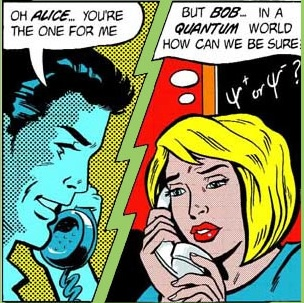
\includegraphics[width=\textwidth]{Quantum_information_image.jpg}
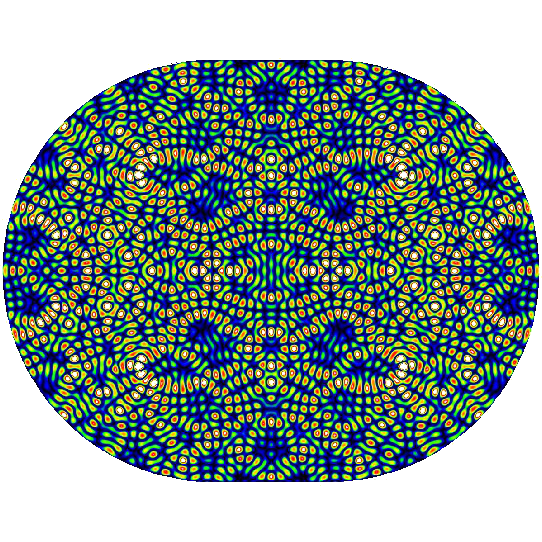
\includegraphics[width=\textwidth]{typicalstadium.png}
\end{minipage}\hfill
\begin{minipage}[l]{\hola}
% \begin{flushleft}
\LARGE
\begin{center}
% \begin{itemize}
\
Información cuántica \\[\spaceitems]
Cadenas de espines \\[\spaceitems]
Matrices aleatorias \\[\spaceitems]
Caos cuántico 
% \end{itemize}
\end{center}
% \end{flushleft}
\end{minipage}
\begin{minipage}[c]{\adios}
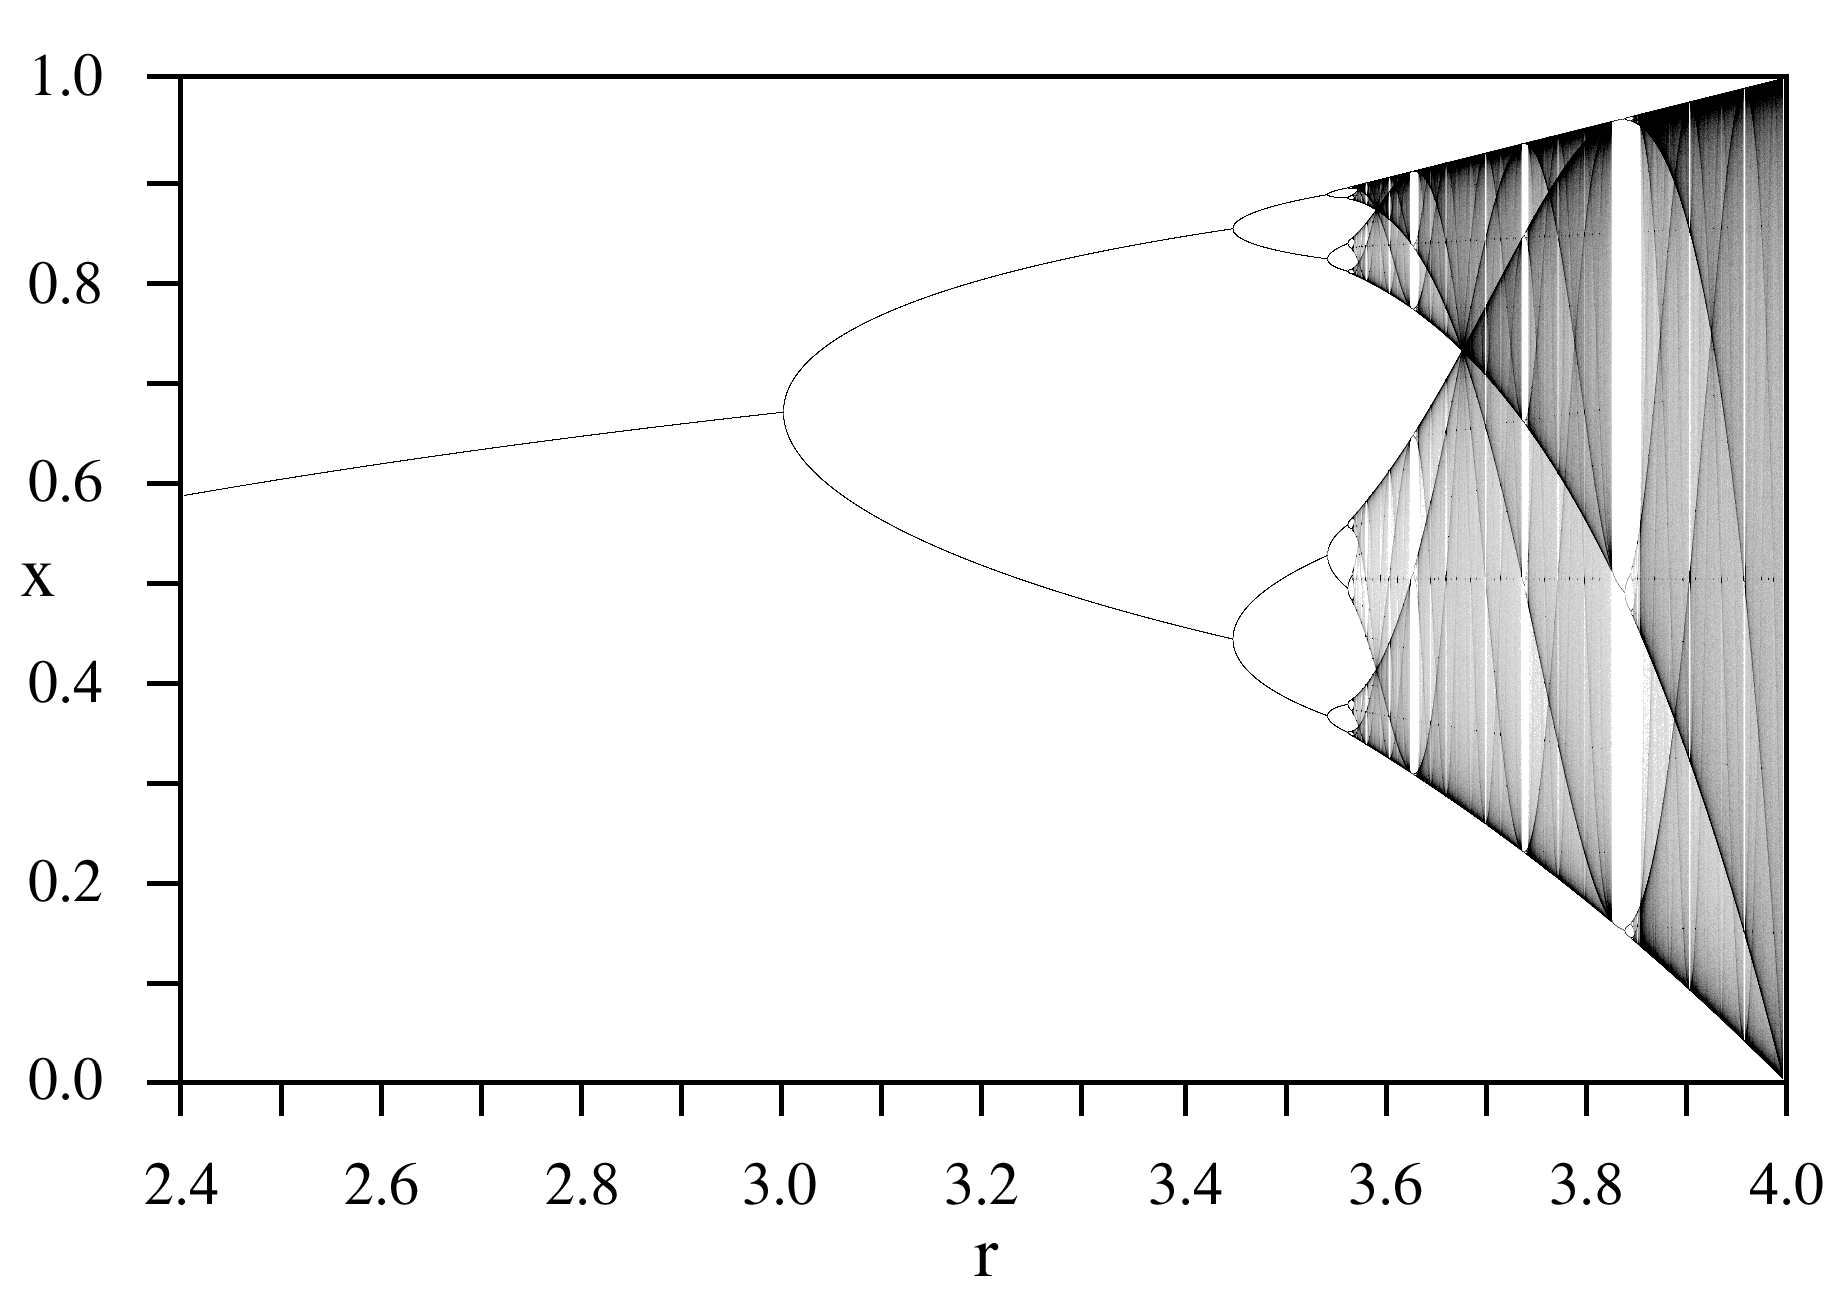
\includegraphics[width=\textwidth]{LogisticMap_BifurcationDiagram2.png}
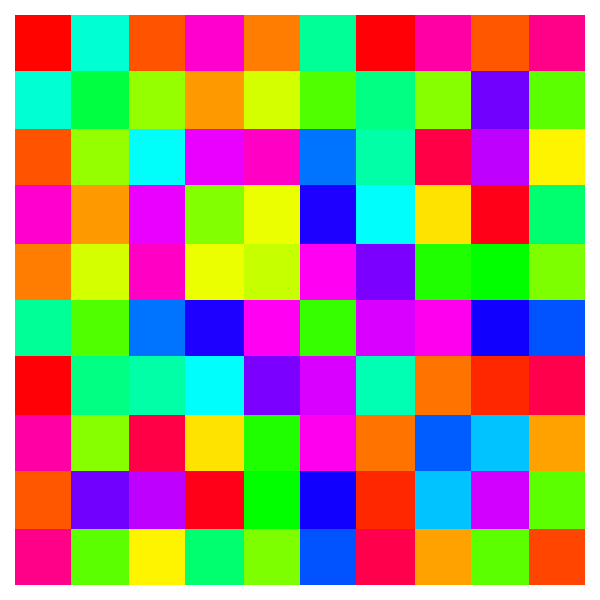
\includegraphics[width=.48\textwidth]{RM1}\hfill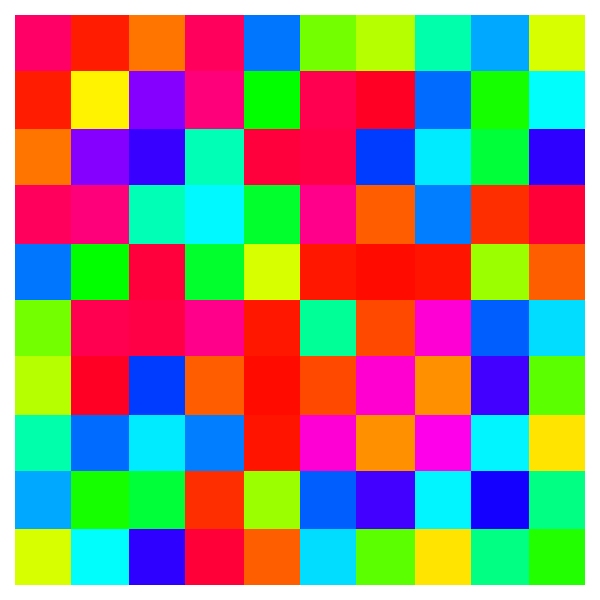
\includegraphics[width=.48\textwidth]{RM2}
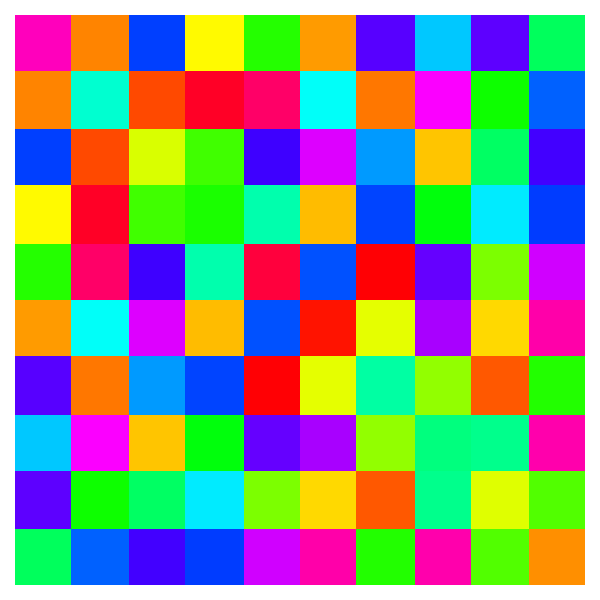
\includegraphics[width=.48\textwidth]{RM3}\hfill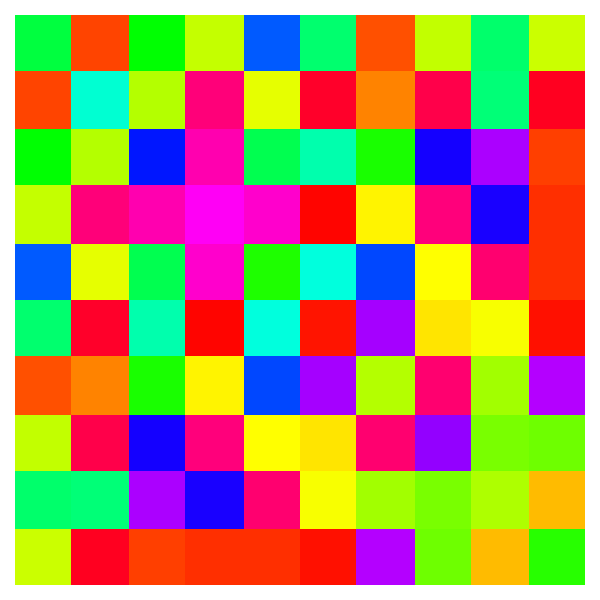
\includegraphics[width=.48\textwidth]{RM4}
\end{minipage}\\[2cm]

\large 
% \parbox{.8\textwidth}{ Se usará Julia para programar, pero el lenguaje hará parte del contenido del curso.  }

\end{center}
% y temas afines. 
\vfill
% Bottom of the page
% {\large \today}

\texttt{
carlosp@fisica.unam.mx \hfill htpp://gioc.fisica.unam.mx
}
\end{titlepage}


\end{document}

